\documentclass{report}
\usepackage{listings}
\usepackage[dvipsnames]{xcolor}
\pagecolor{GreenYellow!10}
\usepackage[utf8]{inputenc}
\usepackage[spanish,mexico]{babel}
\setlength{\textwidth}{18cm}
\setlength{\oddsidemargin}{-1cm}
\setlength{\headsep}{-1cm}
\setlength{\voffset}{0cm}
\setlength{\topmargin}{0cm}
\setlength{\headheight}{0cm}
\usepackage{tikz}
\usetikzlibrary{calc,arrows}
\usepackage{multicol}
\usepackage{lipsum} 

%%%%%% LISTINGS %%%%%%%%%%%%%%%%%%%%%%%%%%%%%%%%%%%%%%%%%
\definecolor{codegreen}{rgb}{0,0.6,0}
\definecolor{codegray}{rgb}{0.5,0.5,0.5}
\definecolor{codepurple}{rgb}{0.58,0,0.82}
\definecolor{backcolour}{rgb}{8.9,8.9,0.9}
\lstdefinestyle{mystyle}{
    backgroundcolor=\color{backcolour},
	commentstyle=\color{codegreen},
	keywordstyle=\color{magenta},
    numberstyle=\tiny\color{codegray},
    stringstyle=\color{codepurple},
    basicstyle=\ttfamily\footnotesize,
    breakatwhitespace=false,         
    breaklines=true,                 
    captionpos=b,                    
    keepspaces=true,                 
    numbers=left,                    
    numbersep=5pt,                  
    showspaces=false,                
    showstringspaces=false,
    showtabs=false,                  
    tabsize=2
}

\lstset{style=mystyle}

\begin{document}
%%%%%% ENCABEZADO %%%%%%%%%%%%%%%%%%%%%%%%%%%%%%%%%%%%%%%
    \begin{minipage}[t]{0.165 \textwidth}
       \begin{flushright}
        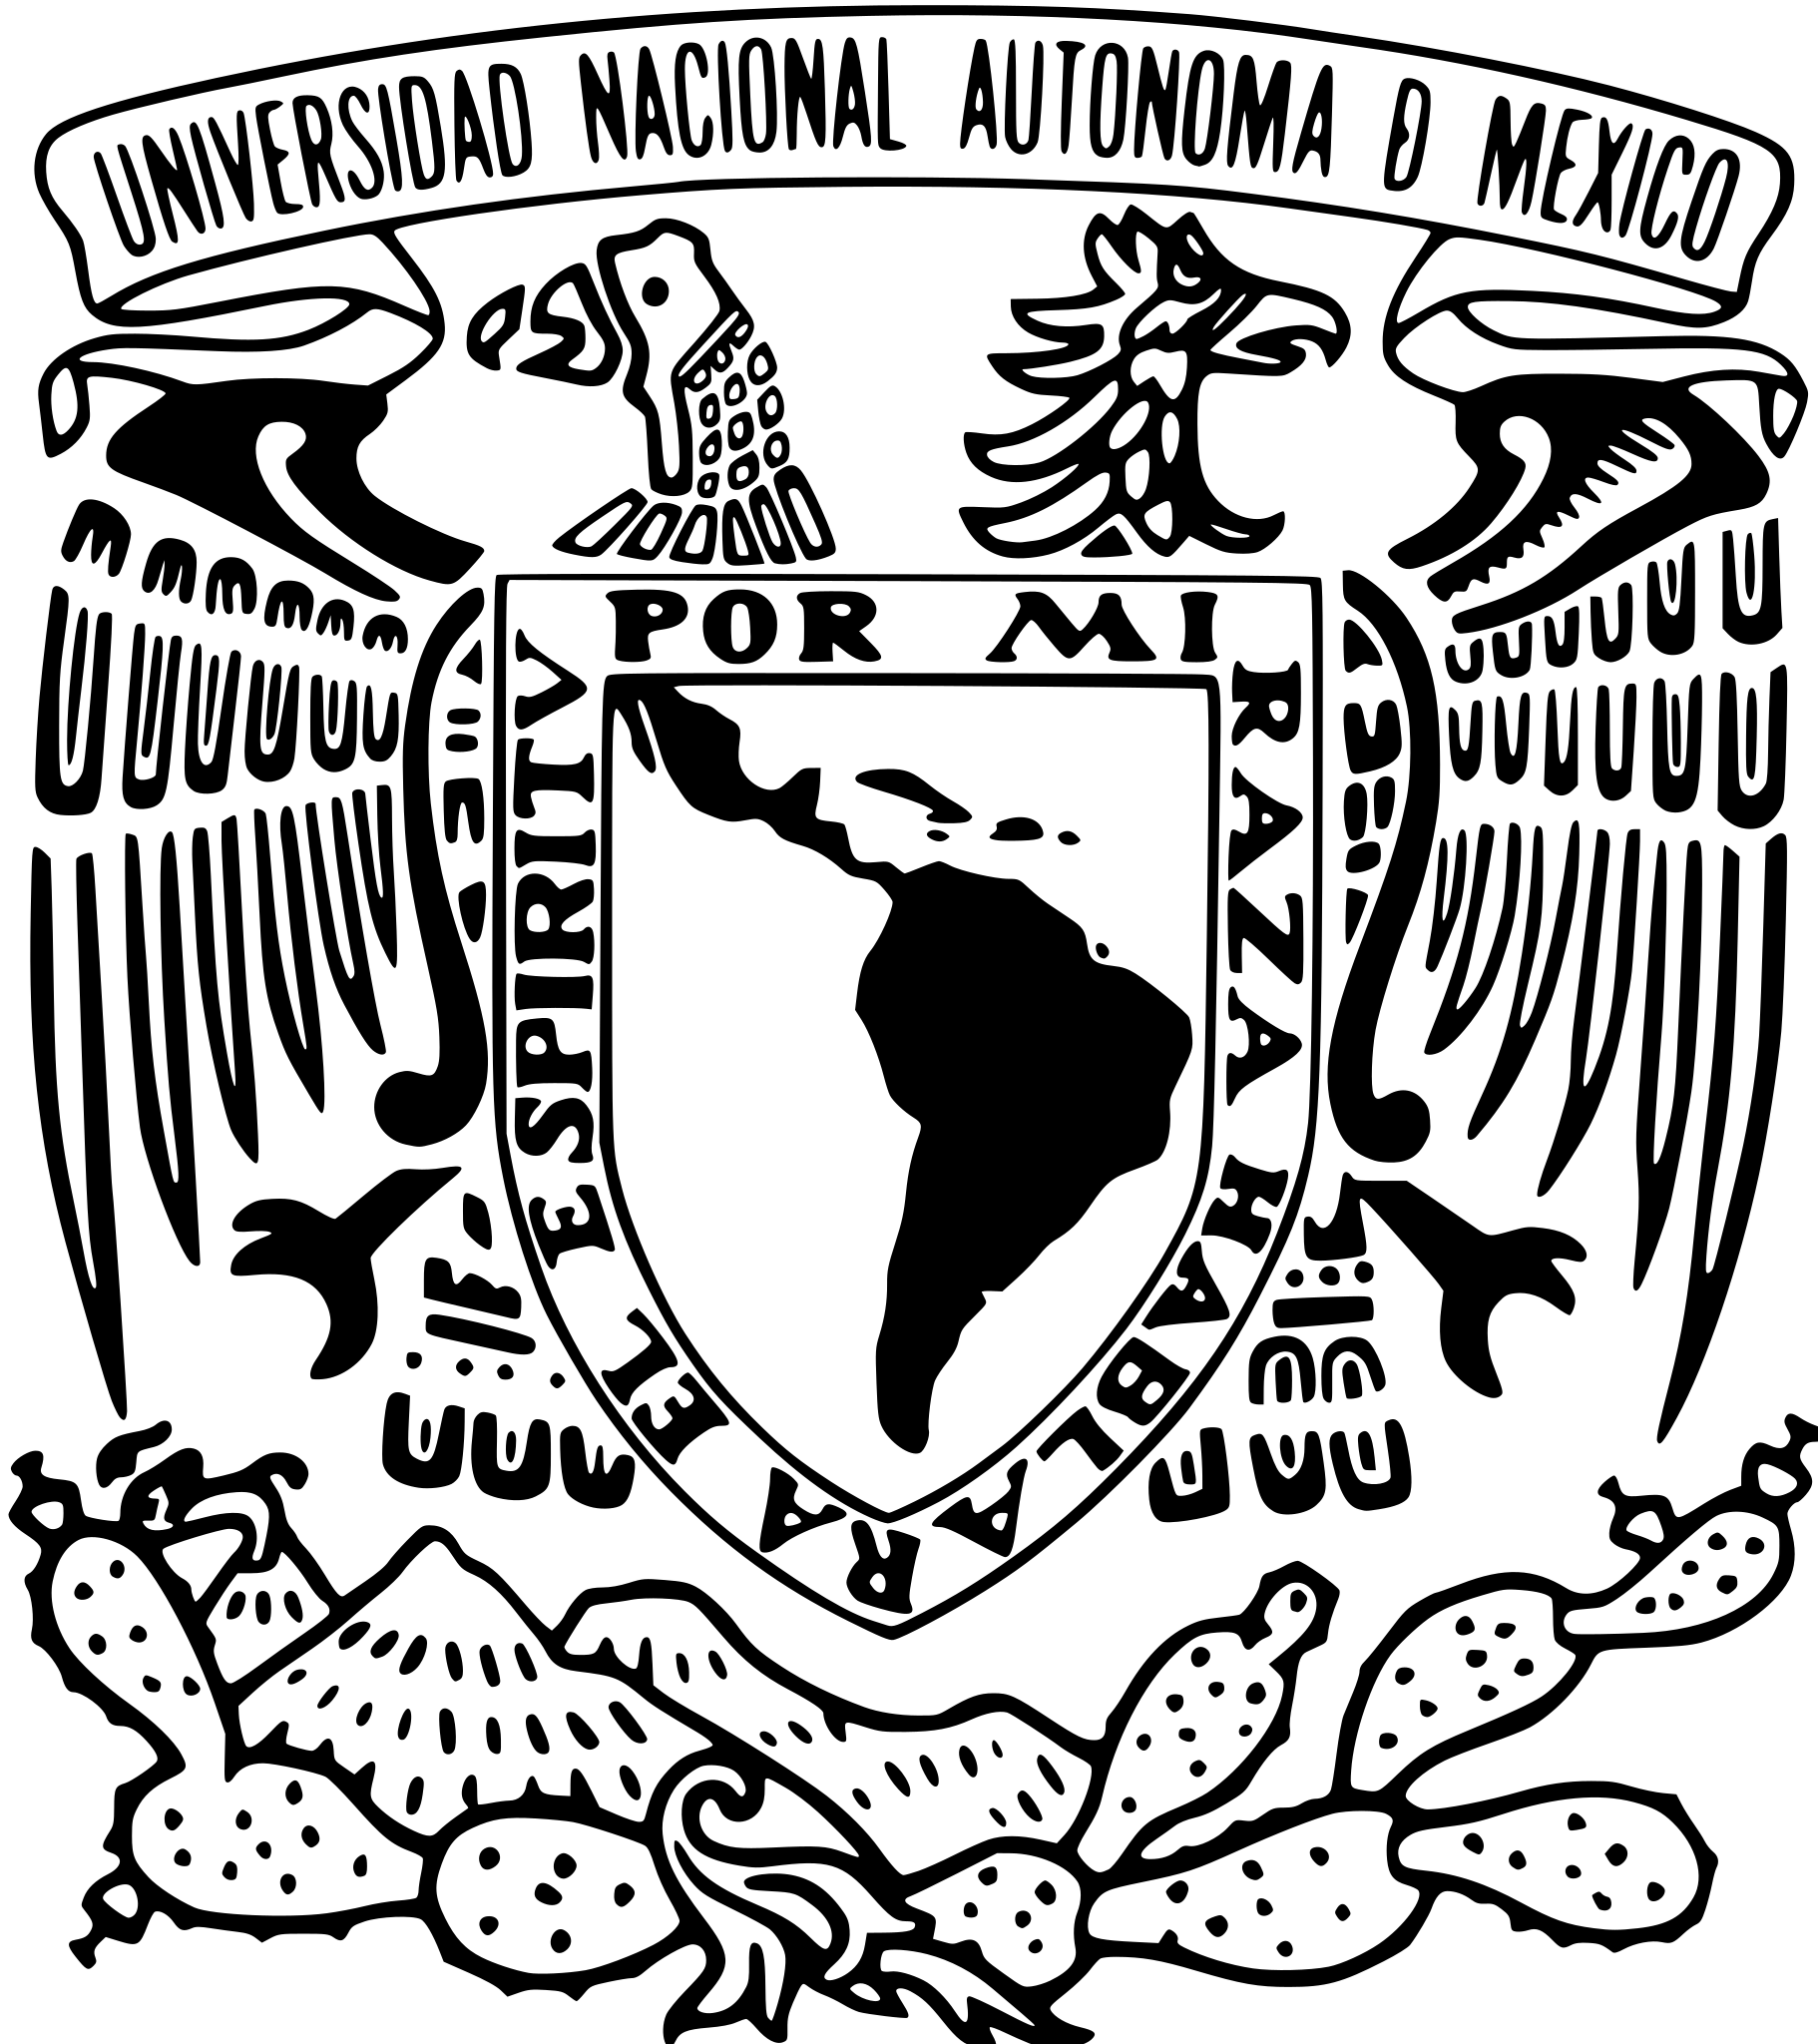
\includegraphics[width=1in]{EscudoUNAM.png}
       \end{flushright}
    \end{minipage}
    \begin{minipage}[H]{0.62 \textwidth}
        \begin{center}
            {\large \textsc{Universidad Nacional Autónoma de México}}
            \vspace{0.25cm}
            \\
            { \huge \textbf{Tarea 3}}
            \\
            \vspace{0.25cm}
            
            \textbf{Introducción a Ciencias de la Computación}
	   		\\
	        \vspace{0.25cm}
	        Rodrigo André Decuir Fuentes
            \vspace{0.2cm}
        \end{center}
        \vspace{0.05cm}
    \end{minipage}
    \begin{minipage}[t]{0.165 \textwidth}
        \begin{flushleft}
            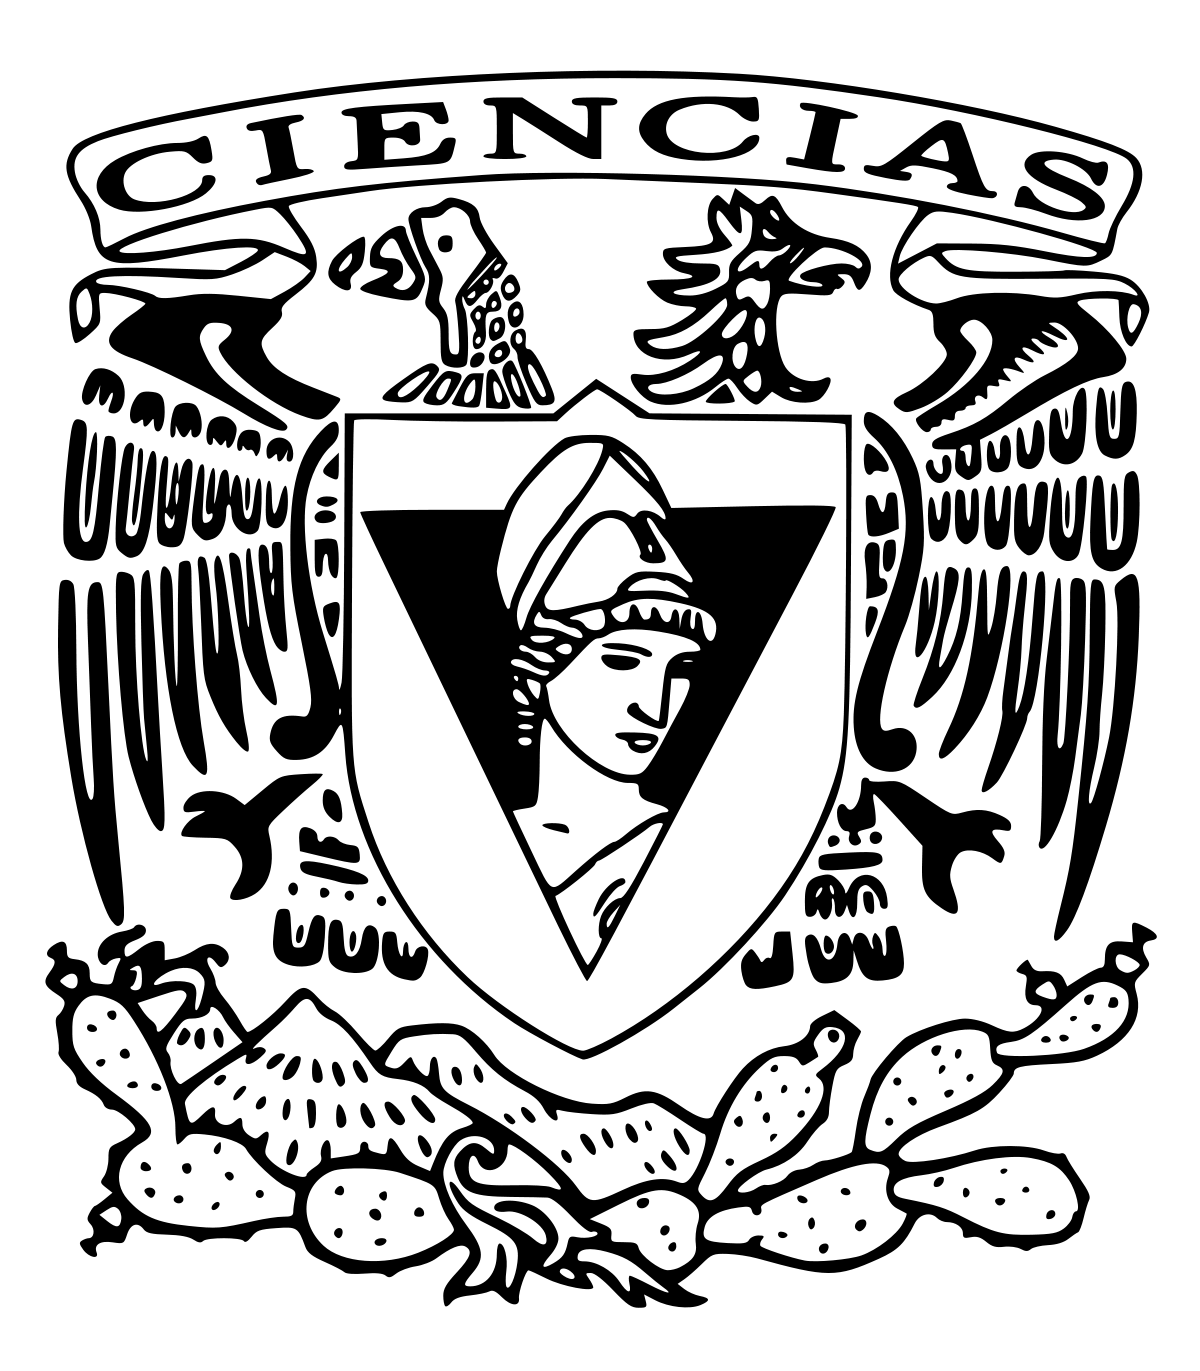
\includegraphics[width=1in]{Fciencias_UNAM.png}
        \end{flushleft}
    \end{minipage}
\begin{tikzpicture}
    \draw[thick] (-6.5,0)--(11.2,0);
\end{tikzpicture}
%%%%%%%%%%%%%%%%%%%%%%%%%%%%%%%%%%%%%%%%%%%%%%%%%%%%%%%%%
\section*{Teoría}
\subsection*{Responde las siguientes preguntas:}
    \begin{enumerate}
	    \item \textbf{¿Qué son los arreglos y para qué son  ́utiles?}
		    \begin{itemize}	
             \item Los arreglos son conjuntos finitos y ordenados de elementos homogéneos, asimismo son objetos.
             \item Son de mucha utilidad para manejar de forma sencilla y directa un conjunto de datos del mismo tipo. 
            \end{itemize}
        \item \textbf{Se tiene el siguiente arreglo:}
            \begin{center}
                \begin{array}{ | *{10}{c |}}
                    \hline
                    2 & 35 & -22 & 0 & 56 & 78 & -84 & 8 & 43 & 1 \\
                    \hline
                \end{array}
            \end{center}
            \newline Ordena el arreglo anterior por medio de Bubble Sort y Selection Sort
            \newline \textbf{Comportamiento Bubble Sort (ejecución):}
            \newline 1. \begin{array}{ | *{10}{c |}}
                    \hline
                    2 & 35 & -22 & 0 & 56 & 78 & -84 & 8 & 43 & 1 \\
                    \hline
            \end{array}
            \newline 2. \begin{array}{ | *{10}{c |}}
                    \hline
                    2 & -22 & 0 & 35 & 56 & -84 & 8 & 43 & 1 & 78 \\
                    \hline
            \end{array}
            \newline 3. \begin{array}{ | *{10}{c |}}
                    \hline
                    -22 & 0 & 2 & 35 & -84 & 8 & 43 & 1 & 56 & 78 \\
                    \hline
            \end{array}
            \newline 4. \begin{array}{ | *{10}{c |}}
                    \hline
                    -22 & 0 & 2 & -84 & 8 & 35 & 1 & 43 & 56 & 78 \\
                    \hline
            \end{array}
            \newline 5. \begin{array}{ | *{10}{c |}}
                    \hline
                    -22 & 0 & -84 & 2 & 8 & 1 & 35 & 43 & 56 & 78 \\
                    \hline
            \end{array}
            \newline 6. \begin{array}{ | *{10}{c |}}
                    \hline
                    -22 & -84 & 0 & 2 & 1 & 8 & 35 & 43 & 56 & 78 \\
                    \hline
            \end{array}
            \newline 7. \begin{array}{ | *{10}{c |}}
                    \hline
                    -84 & -22 & 0 & 1 & 2 & 8 & 35 & 43 & 56 & 78 \\
                    \hline
            \end{array}
            \newline \textbf{Comportamiento Selection Sort (ejecución):}
            \newline 1. \begin{array}{ | *{10}{c |}}
                    \hline
                     2 & 35 & -22 & 0 & 56 & 78 & -84 & 8 & 43 & 1 \\
                    \hline
            \end{array}
            \newline 2. \begin{array}{ | *{10}{c |}}
                    \hline
                    -84 & 35 & -22 & 0 & 56 & 78 & 2 & 8 & 43 & 1 \\
                    \hline
            \end{array}  
            \newline 3. \begin{array}{ | *{10}{c |}}
                    \hline
                    -84 & -22 & 35 & 0 & 56 & 78 & 2 & 8 & 43 & 1 \\
                    \hline
            \end{array}
            \newline 4. \begin{array}{ | *{10}{c |}}
                    \hline
                    -84 & -22 & 0 & 35 & 56 & 78 & 2 & 8 & 43 & 1 \\
                    \hline
            \end{array}
            \newline 5. \begin{array}{ | *{10}{c |}}
                    \hline
                    -84 & -22 & 0 & 1 & 56 & 78 & 2 & 8 & 43 & 35 \\
                    \hline
            \end{array}
            \newline 6. \begin{array}{ | *{10}{c |}}
                    \hline
                    -84 & -22 & 0 & 1 & 2 & 78 & 56 & 8 & 43 & 35 \\
                    \hline
            \end{array}
            \newline 7. \begin{array}{ | *{10}{c |}}
                    \hline
                    -84 & -22 & 0 & 1 & 2 & 8 & 56 & 78 & 43 & 35 \\
                    \hline
            \end{array}
            \newline 8. \begin{array}{ | *{10}{c |}}
                    \hline
                    -84 & -22 & 0 & 1 & 2 & 8 & 35 & 78 & 43 & 56 \\
                    \hline
            \end{array}
            \newline 9.   \begin{array}{ | *{10}{c |}}
                    \hline
                    -84 & -22 & 0 & 1 & 2 & 8 & 35 & 43 & 78 & 56 \\
                    \hline
            \end{array}
            \newline 10.  \begin{array}{ | *{10}{c |}}
                    \hline
                    -84 & -22 & 0 & 1 & 2 & 8 & 35 & 43 & 56 & 78 \\
                    \hline
            \end{array}
    \item \textbf{¿Qué es la recursión y en qué se aplica? ¿Qué componentes debe tener un método recursivo?}
		    \begin{itemize}	
             \item La recursión es la forma de expresar la solución a un problema en términos de sí mismo, es aplicada para trabajar en cosas que tienen muchas ramificaciones posibles y son demasiado complejas para un enfoque iterativo. Un buen ejemplo de esto sería buscar a través de un sistema de archivos. 
             \item Toda función recursiva tiene dos componentes: un caso base y un paso recursivo. 
	        \end{itemize}
    \item \textbf{Se tienen los siguientes dos programas:}
			\newline
            \begin{lstlisting}[language=Java, caption=mist]

  public double mist (int n) {
      double s = 0.0;
      for (double i = 1; i <= n ; i ++) {
             s = s + 1/ i ;
      }
      return s ;
  }	
            \end{lstlisting}
            \begin{lstlisting}[language=Java, caption=mistR]

  public double mistR (int n) {
      if (n <= 1) {
          return 1;
      } else {
          return ((double) 1/ n)  + mistR (n - 1) ;
      } 
  }
            \end{lstlisting}
            \newline ¿Qué hacen mist y mistR?
            \begin{itemize}
                \item \textbf{mist: } recibe un entero, el cual es usado para determinar el número de veces que se va a 
                    realizar la operación de a un número decimal con valor inicial de 0.0 asignarle el valor de ese mismo 
                    número más 1 entre el índice de repetición. Es decir este método realiza un número determinado de veces
                    la operación de sumarse a sí mismo con una mitad cada vez más pequeña de 1. Devuelve lo mismo que $"mistR"$.
                \item \textbf{mistR: } recibe un entero que sirve para determinar el número de veces que se va a realizar la operación. Se tiene un caso base para detener el programa en algún momento, 
                    en el caso de la operación, esta realiza lo mismo $"mist"$ pero de forma recursiva, es decir, 
                    se divide entre 1 entre un número n y a esto se le suma el antecesor de $"mistR"$ usando $"mistR"$. Devuelve lo 
                    mismo que $"mist"$.
            \end{itemize}
            \newline ¿Cuál de las dos versiones es mejor y por qué?
            \newline La mejor versión es \textbf{mist}, ya que la iteración en este caso es más rápida que la recursión y dado que estamos 
            trabajando con un double, tenemos que el resultado es cada vez más dificil de controlar, incluso si le pasamos 
            un valor $'n'$ muy grande a ambos métodos, por poner un ejemplo 100000, el método iterativo va a terminar muy rápido, mientras
            que el recursivo probablemente entre en $"STACKOVERFLOW"$, lo que significa que la iteración en este caso no permite manejar
            más números que la recursión.
    \item \textbf{¿Por que es tan importante la Complejidad en Ciencias de la Computación?}
			    \newline Es importante porque nos permite determinar la eficacia de un algoritmo. La cual se expresa en función del tamaño de la entrada.
                Para poder representar la complejidad se hace uso de la notación O grandota la cual permite evaluar el ritmo de crecimiento
                en el tiempo de ejecución como una función dependiente de la cantidad de datos.
	\item \textbf{Se tiene el siguiente programa:}	
            \begin{lstlisting}[language=Java, caption=mist]
            
  public int mist (int n) {
      int r ;
      for (r = 0; n != 0; n /= 10) {
          r += n % 10;
      }
      return r ;
  }
            \end{lstlisting}
            \begin{lstlisting}[language=Java, caption=mistR]
            
  public int mistR (int n)  {
      if (n == 0) {
          return 0;
      } else {
          return (n % 10) + mistR (n / 10) ;
      }
  }
            \end{lstlisting}
        \newline ¿Cuál es la complejidad de mist y mistR? Justifica tu respuesta.
        \begin{itemize}
            \item \textbf{mist: $O(n)^2$}  Operación: O(1) + ( 
            \item \textbf{mistR: $O( ) $}  Operación: ( )  
        \end{itemize}
        \newline ¿Cuál método utiliza la regla de suma y cuál la regla de la multiplicación?
        \begin{itemize} 
            \item $"mist"$ utiliza la regla de la suma y $"mistR"$ la regla de la multiplicación.
        \end{itemize}
    \end{enumerate}
\end{document}
